\documentclass{article}
\usepackage[left=2cm, right=2cm, top=2cm]{geometry}
\usepackage[utf8]{inputenc}
\usepackage{amsmath}
\usepackage{graphicx}

\title{Home Assignment 1}
\author{André Hedesand}
\date{October 2018}

\begin{document}

\maketitle
\section*{Foreword}
If there is something fishy about my calculations, you can probably and hopefully
find it in the Collection of Formulas.

\section*{Solutions}

\begin{enumerate}
    \item % 1
        \begin{enumerate}
            \item % 1a
                \emph{"Recursive systems are never stable"}
                \\
                \textbf{False.} 
                Recursive systems are IIR systems e.g. 
                $$ y(n) = \frac{1}{2}y(n-1) + x(n) $$
                If we by stability mean BIBO-stability we can simply prove that the system above is stable. The Z-transorm of the system above is
                $$ 
                    Y(z) = \frac{1}{2}z^{-1}Y(z) + X(z) \Rightarrow
                    Y(z)(1 - \frac{1}{2}z^{-1}) = X(z) \Rightarrow
                $$
                $$
                    Y(z) = \frac{1}{1 - \frac{1}{2}z^{-1}}X(z) = 
                    H(z) X(z) \Rightarrow 
                    H(z) = \frac{1}{1 - \frac{1}{2}z^{-1}} \longmapsto
                $$
                $$
                    h(n) = (\frac{1}{2})^{n} u(n)
                $$
                
                By definition the system above is stable if
                $ \sum_{n=0}^{\infty} |(\frac{1}{2})^{n}| < \infty $.
                This is true because $(\frac{1}{2})^{n}$ goes to zero when $n$
goes to $\infty$, which means that the sum converges.
            
            \item % 1b
                \emph{"A convolution of two sequences in the time domain corresponds to a multiplication of the Z transforms of the signals."}
                \\
                \textbf{True.} If we look at the definition and the
                statement:
                \\
                \begin{align*}
                    \begin{tabular}{c l}
                        Statement: & $a(n) = b(n)*c(n) \longmapsto A(z) = B(z)C(z)$ \\
                        Defenitions: & $b(n)*c(n) = \sum_kb(k)c(n-k)$ \\
                         & $A(z) = \sum_na(n)z^{-n}$ \\
                    \end{tabular}
                \end{align*}
                Lets start with the last defenition:
                $$
                    A(z) = \sum_na(n)z^{-n} = \sum_n \left[ \sum_kb(k)c(n-k) \right]z^{-n}
                    = \sum_kb(k) \left[ \sum_nc(n-k) \right] z^{-n}z^{k}z^{-k} 
                $$ $$
                = \sum_kb(k)z^{-k} \sum_nc(n-k)z^{-(n-k)} = B(z) C(z)
                $$
            \item % 1c
                \emph{"An FIR filter is always stable."}
                \\
                \textbf{True.}
                A FIR filter is always \emph{BIBO stable} and can be discribed
                with a difference equation:
                $$ 
                y(n) = \sum_{k=0}^{N} a_k x(n-k)
                $$
                The system is always stable as every 
                $a_n < \infty$ 
                and 
                $N<\infty$
                
            \item % 1d
                \emph{"A first order IIR filter is stable iff the absolute value of the value of the factor in front of $y(n-1)$ is greater than 1."}
                \\
                \textbf{False.} The opposite is true. We can prove this by
                contradiction: If we assume the statement above is true we get
                the following:
                
                $$
                    y(n) = Ay(n-1) + x(n), A > 1
                $$
                \begin{center}
                    \textit{and}
                \end{center}
                $$
                   \sum_k |h(k)| < \infty
                $$
                Here $A$ denotes the \emph{"factor in front of $y(n-1)$"}.
                
                Lets do the same steps as in \emph{1a)}:
                $$
                   y(n) = Ay(n-1) + x(n) \Rightarrow h(n) = A^nu(n)
                $$
                At last we get
                $$
                  \sum_k |h(k)| < \infty \Leftrightarrow \sum_{n=0}^{\infty}|A^n| < \infty,  (A > 1)
                $$
                Which can't be true as the sum $\sum_{n=0}^{\infty}|A^n|
\rightarrow \infty$ as $A>1$.
                
            \item % 1e
                \emph{"An IIR-filter is never a linear-phase system."}
                % TODO
                
                {\Large \centering INTE KLAAAAAAAAAAR}
                
                
        \end{enumerate} % 1abcde
    \item % 2
        \emph{"A discrete-time system is described by the difference equation:"}
        $$
            y(n)-y(n-1) + \frac{2}{9}y(n-2) = x(n)
        $$
        \begin{enumerate}
            \item % 2a
                \emph{"Determine the system function $H(z)$ and the impulse response $h(n)$ for the system and draw a pole-zero plot. Is the system stable?"}
                
                $$
                    y(n)-y(n-1) + \frac{2}{9}y(n-2) = x(n) \longmapsto 
                    Y(z) - Y(z)z^{-1} + \frac{2}{9} Y(z)z^{-2} = X(z) \Rightarrow
                $$ $$
                    Y(z)(1 - z^{1} + \frac{2}{9} z^{-2}) = X(z) \Rightarrow
                    Y(z) = \frac{1}{1 - z^{-1} + \frac{2}{9}z^{-2}} X(z) = H(z)X(z)
                $$
                
                Now we have the system function. To get the impulse response we just need to inverse transform the system function.
                $$
                    H(z) = \frac{1}{1 - z^{-1} + \frac{2}{9}z^{-2}} = 
                    \frac{z^2}{z^2 - z + \frac{2}{9}} = 
                    \frac{z^2}{ (z-\frac{2}{3}) (z-\frac{1}{3}) } = 
                    1 + \frac{z-\frac{2}{9}}{ (z-\frac{2}{3}) (z-\frac{1}{3}) } =
                $$ $$
                    \left\{ PF \right\} 
                    1 + \frac{\frac{4}{3}}{z-\frac{2}{3}} - \frac{\frac{1}{3}}{z-\frac{1}{3}} = 
                    1 + z^{-1}\frac{\frac{4}{3}}{1-\frac{2}{3}z^{-1}}
                    - z^{-1}\frac{\frac{1}{3}}{1-\frac{1}{3}z^{-1}} 
                $$ $$
                    \longmapsto h(n) = \delta(n) + \frac{4}{3} \left( \frac{2}{3} \right)^{n-1}u(n-1)
                    - \frac{1}{3}\left( \frac{1}{3}\right)^{n-1}u(n-1) 
                    = \delta(n) + \left( 2 \left( \frac{2}{3} \right)^n
                    - \left( \frac{1}{3} \right)^n \right) u(n-1)
                $$
               	\begin{figure*}[h]
               		\centering
               		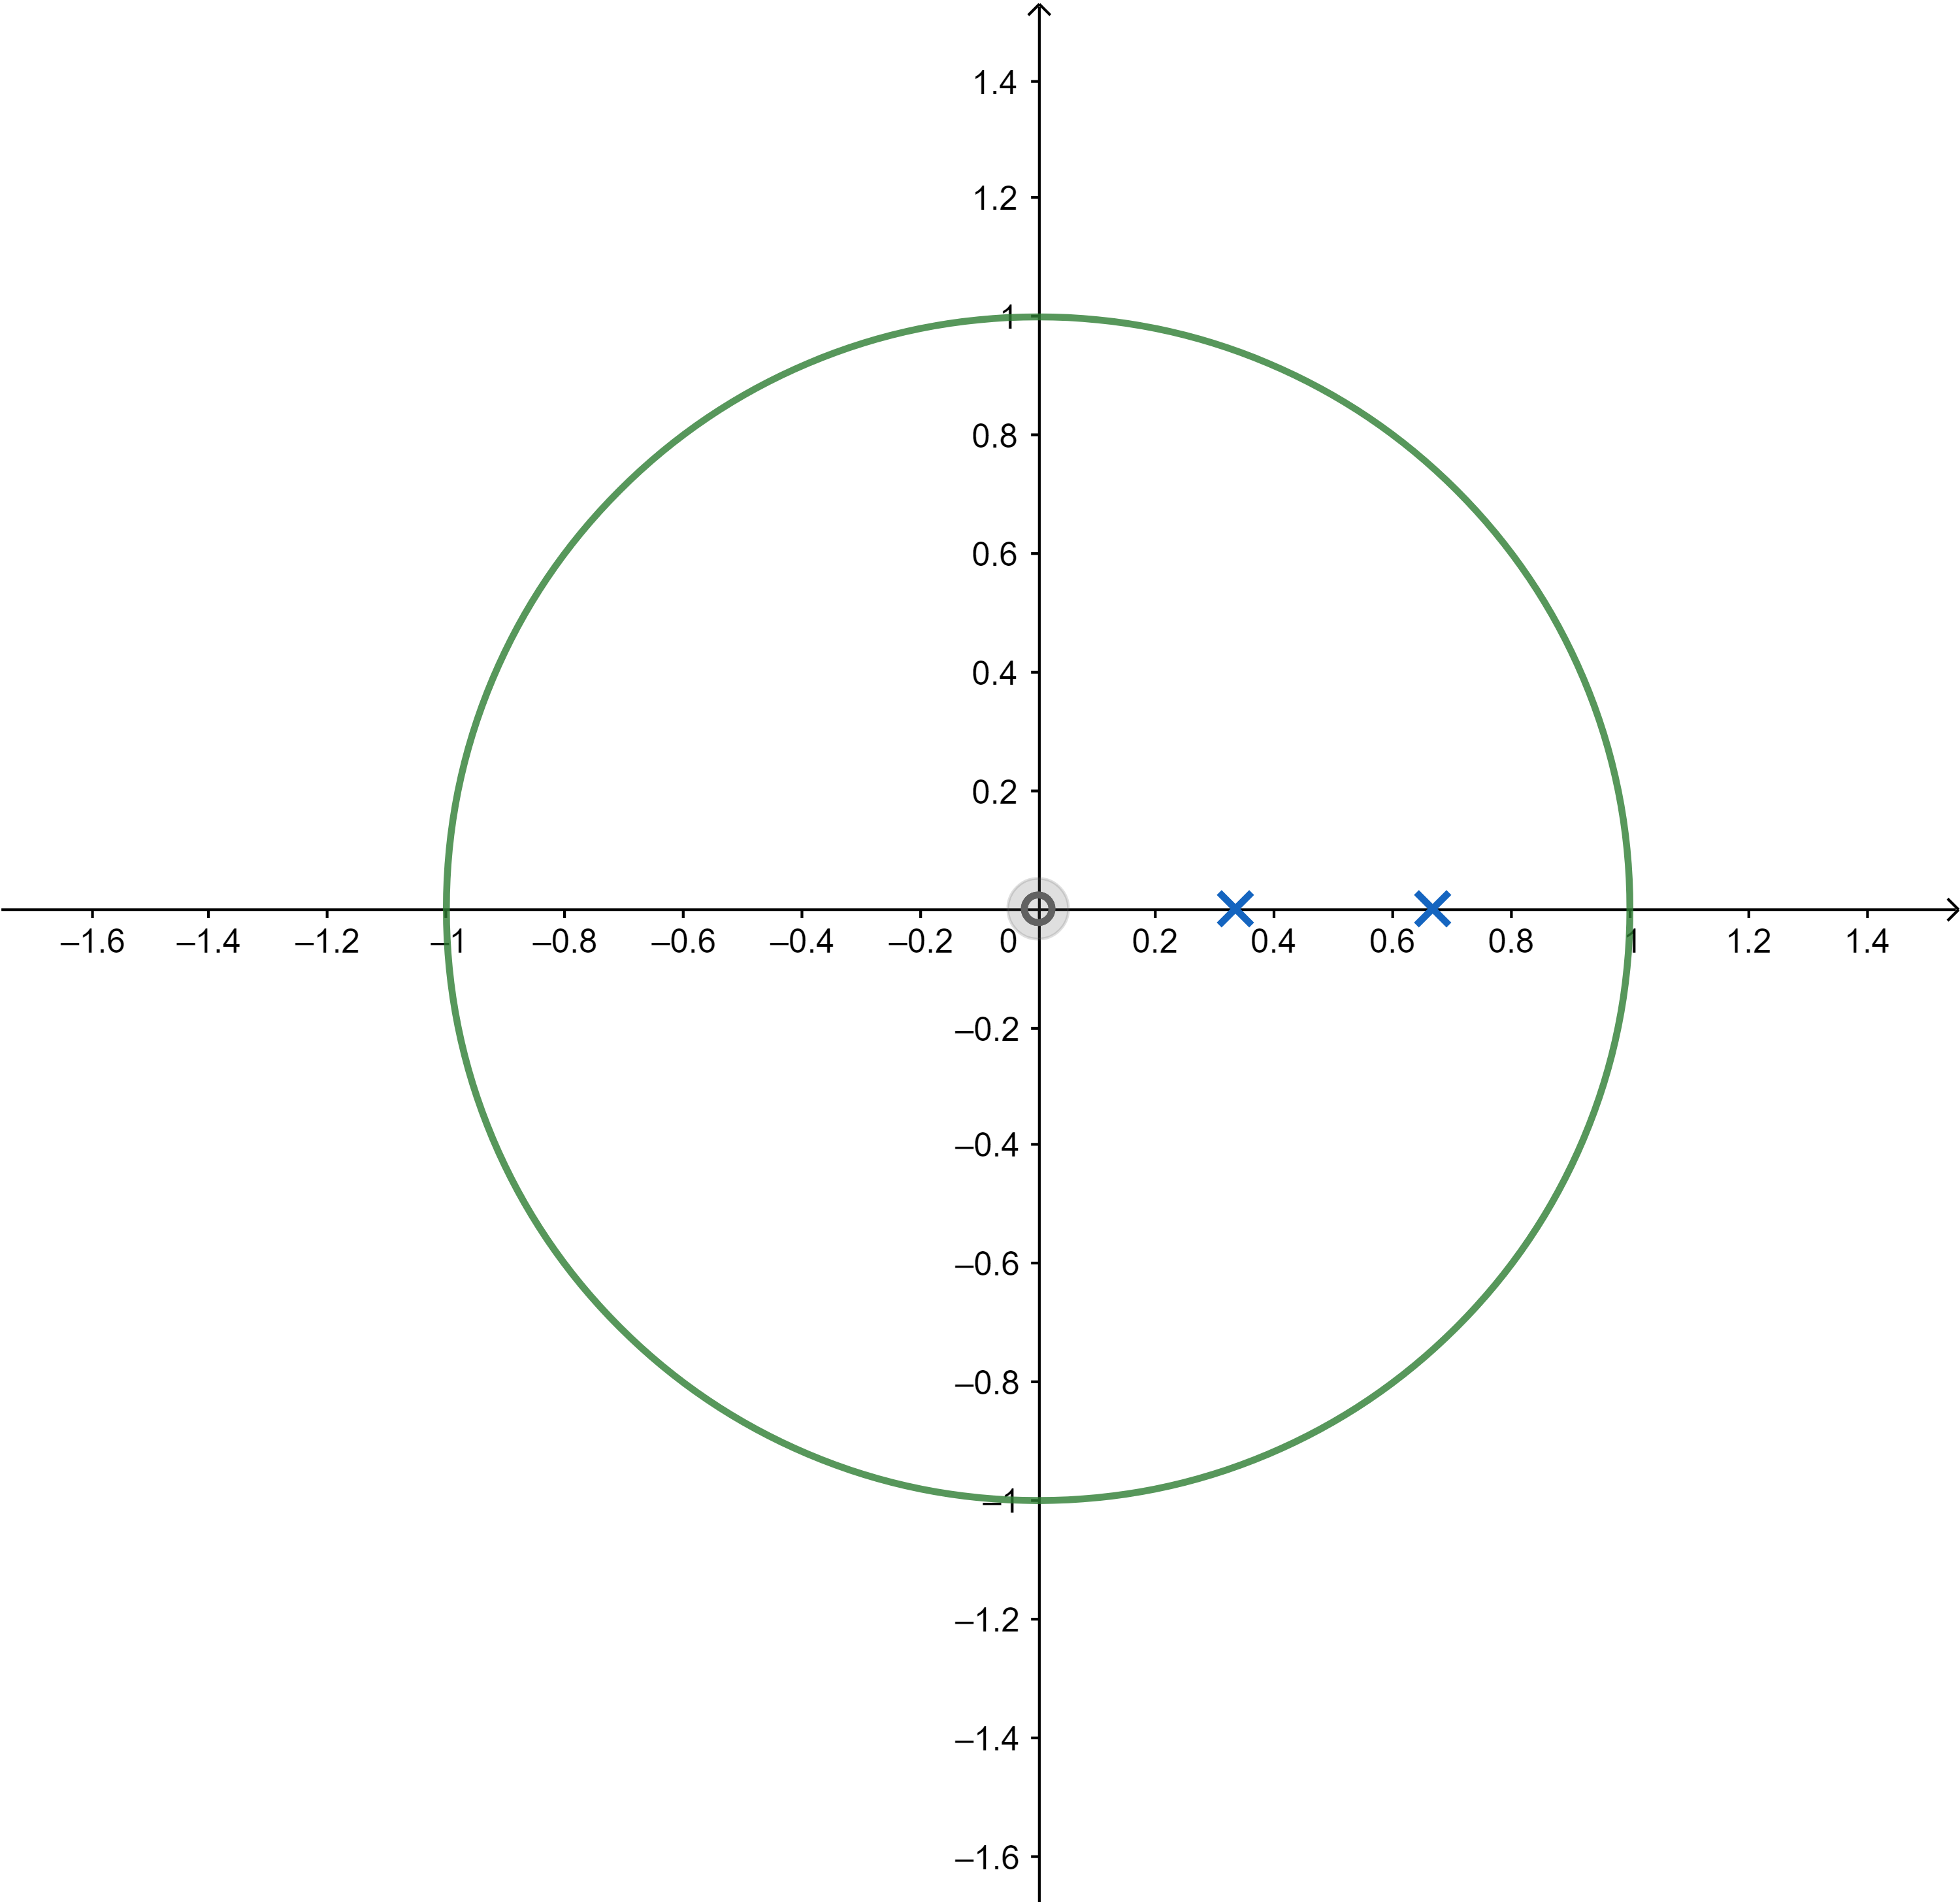
\includegraphics[width=8.0cm]{geogebra-export.png}
               		\caption{Poles and zeros of the system}
               		\label{fig:plot1}
               	\end{figure*}

                We can see that the system is stable in 2 ways: On the impulse
response, where the potents of $n$ is $<1$ and in the graph, where the poles
are inside the unit circle.
                
                
                
            \item % 2b
                \emph{"The following signal is the input signal to the system"}
                $$
                    x(n) = 3(\frac{1}{2})^nu(n)
                $$
                \textit{"where u(n) is the step function. Solve the difference equation by using the Z-transform, that is, determine a closed form expression for y(n)."}
                \\
                We know by definition that the output from the system is equal to the
                convolution of the input and the impulse response. 
                $$
                    y(n) = h(n) * x(n) \Longleftrightarrow Y(z) = H(z) X(z)
                $$
                When $Y(z)$ is calculated, we've got our answer. $X(z) = 3\frac{1}{1-\frac{1}{2}z^{-1}}$
                $$
                    H(z) X(z) = \frac{1}{(1-\frac{1}{3}z^{-1})
                    (1-\frac{2}{3}z^{-1})} * 3\frac{1}{1-\frac{1}{2}z^{-1}}
                    = \left\{ PF \right\}
                    \left( -\frac{8}{5}  \right) \frac{1}{1-\frac{1}{3}z^{-1}}
                    + \frac{22}{5} \frac{1}{1-\frac{2}{3}z^{-1}}
                    - \frac{14}{5} \frac{1}{1-\frac{1}{2}z^{-1}} \longmapsto
                $$

                $$
                    \longmapsto 
                    y(n) = 
                    \left(
                        \frac{22}{5}
                        \left(
                            \frac{2}{3}
                        \right)^n
                        -
                        \frac{8}{5}
                        \left(
                            \frac{1}{3}
                        \right)^n
                        -
                        \frac{14}{5}
                        \left(
                            \frac{1}{2}
                        \right)^n
                    \right)
                    u(n)
                $$

                We can se that the system is stable as every base in the
                potents of $n$ are less than 1.
        \end{enumerate}
    \item % 3
        \emph{"The figures below show four pole-zero plots and four impulse responses."}
        \begin{enumerate}
            \item % 3a
                \emph{"Pair the correct plot A, B, C, D with the corresponding impulse response 1, 2, 3, 4."}
                \\
                \begin{center}
                    \begin{tabular}{c|c}
                        A & 1 \\
                        B & 3 \\
                        C & 4 \\
                        D & 2 \\
                    \end{tabular}
                \end{center}
            \item % 3b
                \emph{"Pair the correct plot A, B, C, D with the corresponding statement I, II, III, IV."}
                \\
                \begin{center}
                    \begin{tabular}{c|c}
                        A & I \\
                        B & III \\
                        C & II \\
                        D & IV \\
                    \end{tabular}
                \end{center}
                
                
        \end{enumerate} % 3ab
        
	\end{enumerate} % 1,2,3
\end{document}
